\recipe{Belle's Filled Pittas}
\label{recipe:filled_pittas}
\makes{x portions}
\worktime{\SI{10} \minute}
\totaltime{\SI{10} \minute}
\source{\href{https://www.bbcgoodfood.com/}{short link to source}}


\begin{ingredients}

\ingroup{For the Flatbreads}
	\item \SI{200}{\gram} self-raising flour
	\item \SI{170}{\gram} greek yoghurt
\ingroup{For The Filling}
	\item \SI{100}{\gram} feta, crushed
	\item \SI{2}{\tablespoon} cream cheese
	\item Handful of mint leaves, finely chopped
	\item \SI{100}{\gram} spinach, wilted with boiling water, squeezed and roughly chopped
	\item 2 garlic cloves, minced
	\item \SI{1}{\teaspoon} black pepper

\end{ingredients}


\begin{method}
	In a large bowl, add in flour and Greek yoghurt. Mix and then knead
for 5 minutes. Add more flour if the dough is too sticky. Cover with
cling film and set aside while you make your filling.

Place all filling ingredients into a bowl and combine thoroughly
(make sure water is squeezed out of spinach). Set aside.

Once your dough has rested, knead it again for 30 seconds and then
slice into 4 equal-sized pieces.

Take one dough ball and flatten with your fingers until about ¾ inch
thick. Place a large tablespoon of the filling into the centre of the
dough and then bring in all the corners of the dough into the centre,
around the feta mixture, and seal the parcel. Turn the parcel over
face down and flatten out the dough with your fingers until the
flatbread is around ½ inch thick. Set aside with a sprinkle of flour.

Place a non-stick dry pan on medium to high heat.

Gently place your flatbreads into the pan and fry for 3-5 minutes on
each side. Flip them over when they go golden-brown
  
\end{method}




\begin{figure}[h]
  \centering
  
  \begin{minipage}{0.48\linewidth}
  	\centering
	\begin{tikzpicture}
  		% Save the image in a box to get its dimensions
  		\sbox0{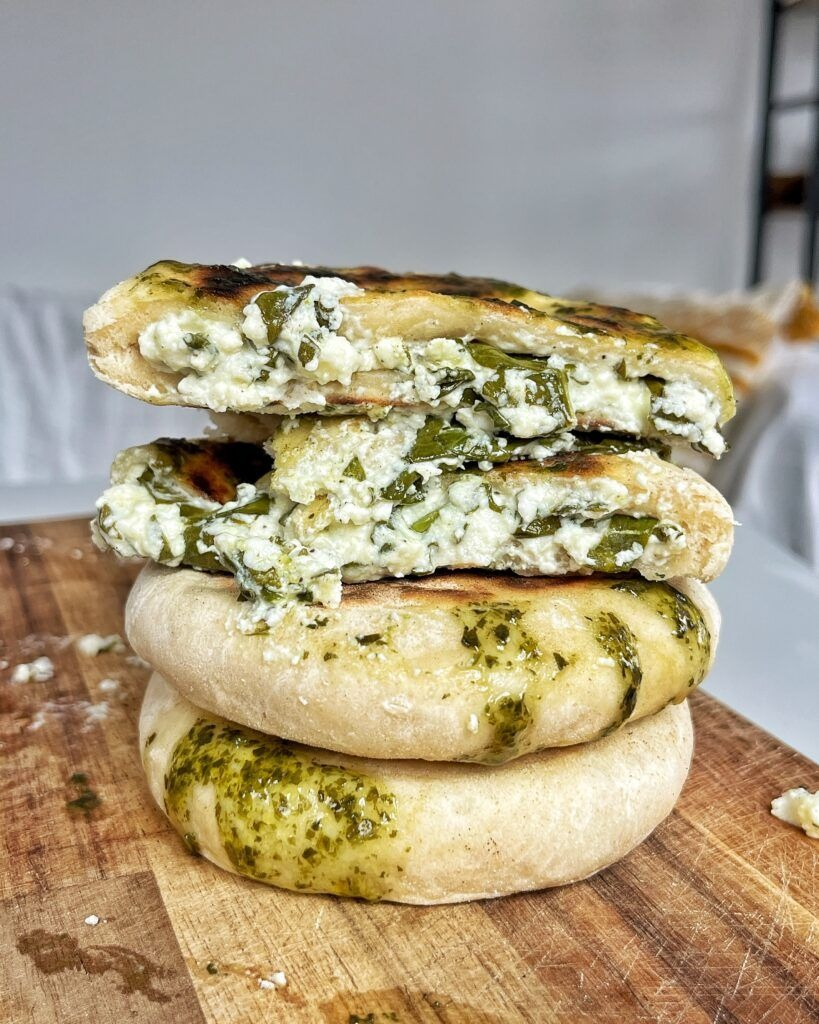
\includegraphics[width = 0.6\linewidth]{images/bellesPittas.jpeg}}%
  
  		% Draw a clipping rectangle with rounded corners
  		\path[clip, rounded corners=0.5cm] (0,0) rectangle (\wd0,\ht0);
  
  		% Place the image inside the clipped area
  		\node[inner sep=0pt, outer sep=0pt, anchor=south west] at (0, 0) {\usebox0};
	\end{tikzpicture}
  \end{minipage}
  \hfill
  \begin{minipage}{0.48\linewidth}
  	\centering
	\begin{tikzpicture}
  		% Save the image in a box to get its dimensions
  		\sbox0{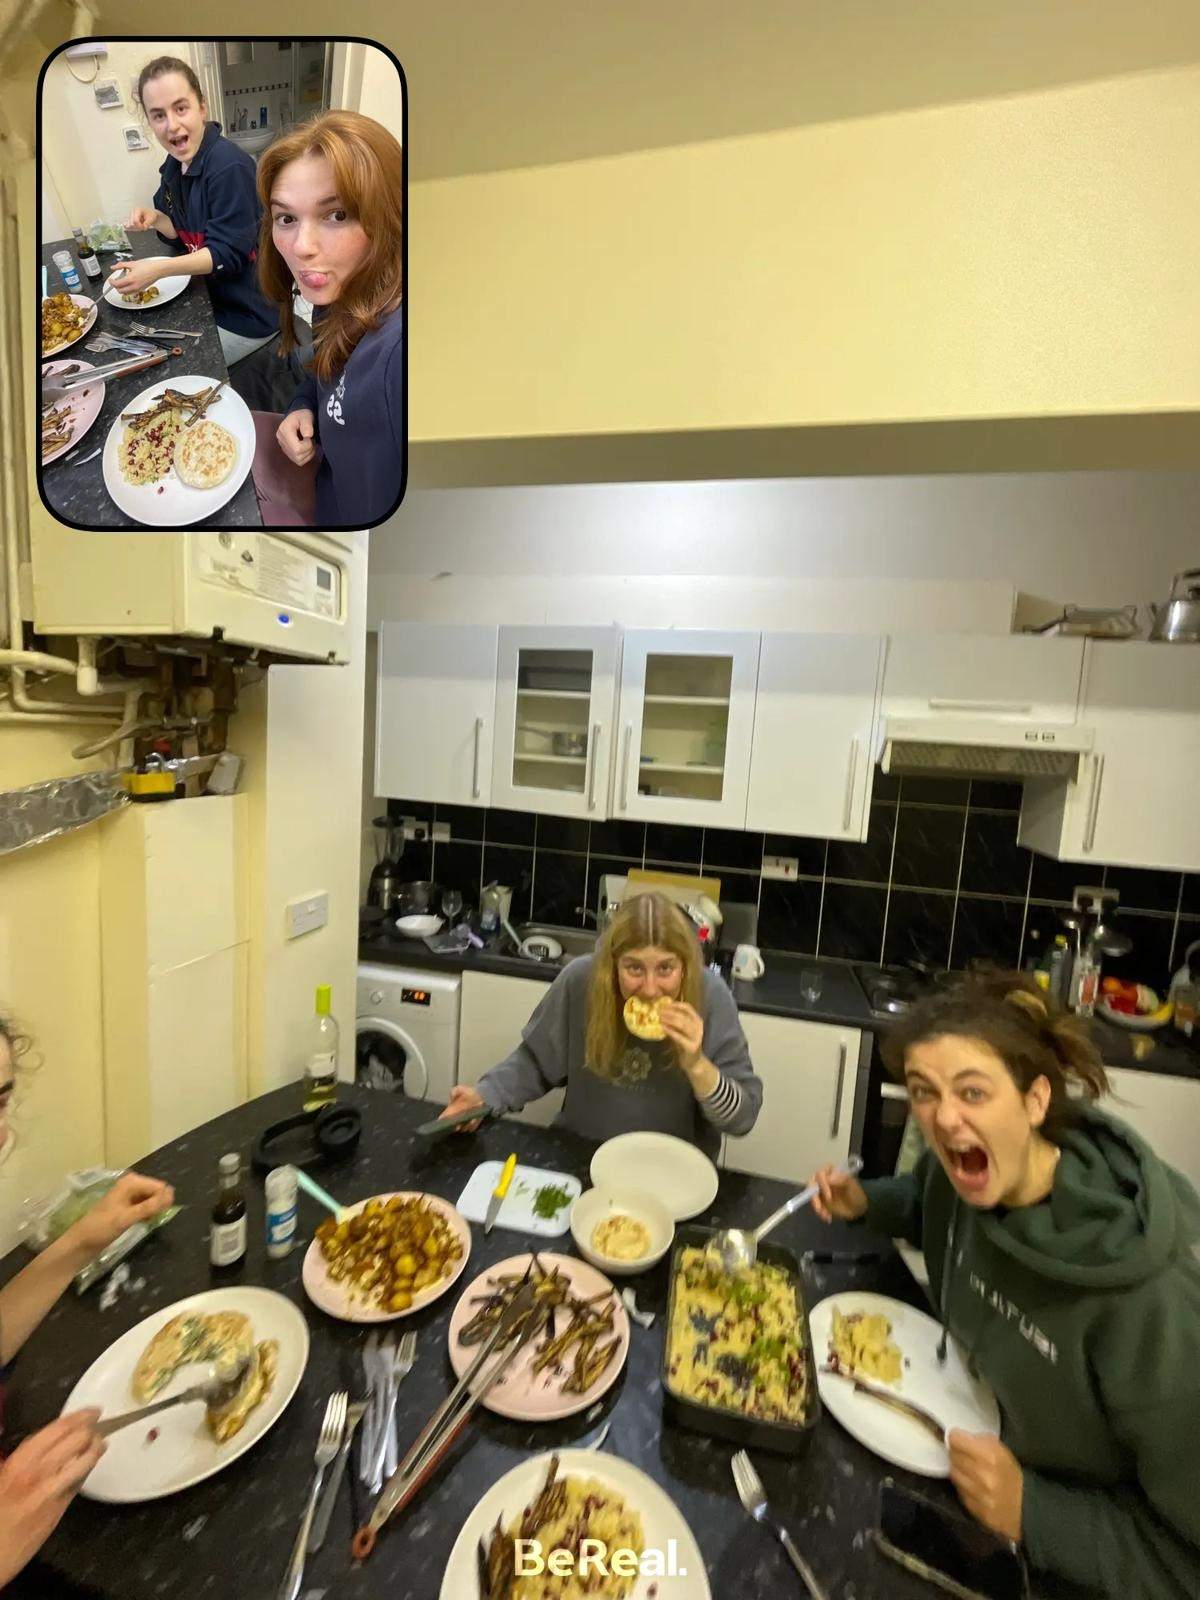
\includegraphics[width = 0.55\linewidth]{images/bellesPittasBeReal.jpeg}}%
  
  		% Draw a clipping rectangle with rounded corners
  		\path[clip, rounded corners=0.5cm] (0,0) rectangle (\wd0,\ht0);
  
  		% Place the image inside the clipped area
  		\node[inner sep=0pt, outer sep=0pt, anchor=south west] at (0, 0) {\usebox0};
	\end{tikzpicture}
  \end{minipage}
\end{figure}

\begin{notes}
Optional serve with mint sauce mixed with olive oil
\end{notes}

